\onehalfspacing
\fancypagestyle{plain}{
\fancyhf{}
\rhead{\thepage}
\renewcommand{\headrulewidth}{0pt}
\renewcommand{\footrulewidth}{0pt}
}

\chapter{PLANTEAMIENTO}

\section{Antecedentes}

El panorama energético global se encuentra en una fase de transformación estructural con el objetivo de alcanzar el escenario de \textit{Net Zero Emissions} (NZE) para el año 2050. Dentro de este marco, se proyecta un crecimiento masivo de la demanda eléctrica global, fuertemente impulsada por la rápida electrificación de usos finales que anteriormente dependían de combustibles fósiles, destacando especialmente la industria y el transporte \citep{IEA_NZE_2021}. Para cubrir esta acelerada demanda eléctrica sin incrementar las emisiones, las energías limpias asumen un rol indispensable; específicamente, la energía solar fotovoltaica y la eólica deben cuadruplicar su ritmo de despliegue histórico, requiriendo alcanzar adiciones anuales de 630 GW de energía solar y 390 GW de energía eólica para el año 2030 \citep{IEA_NZE_2021}. 

De acuerdo con la hoja de ruta de la Agencia Internacional de Energía (IEA), este escenario marca el inicio de una era dominada por las energías limpias, donde el consumo eléctrico escala mientras que el suministro de energía primaria proveniente de combustibles fósiles cae del 80\,\% en 2020 a poco más del 20\,\% en 2050 (Véase Figura \ref{fig:TendenciasNZE2050}). A pesar de que la energía solar y eólica se convierten en los pilares del sistema, la inversión anual en energía limpia debe aumentar desde los niveles actuales hasta alcanzar los 4 billones de dólares para 2030 \citep{IEA_NZE_2021}. Esta transición requiere superar cuellos de botella críticos, especialmente en la expansión y modernización de las redes eléctricas, cuya inversión anual debe duplicarse para evitar deficiencias en el balance energético y asegurar la integración de la generación variable, minimizando así el desperdicio forzado de energía limpia \citep{IEA_WEO_2025}.

\begin{figure}[H]
	% Fuerza la alineación izquierda y quita los ":" después del número
	\captionsetup{justification=raggedright, singlelinecheck=false, labelsep=none}
	
	\caption[Tendencias de la demanda energética proyectadas al 2050 bajo el escenario de Net Zero Emissions.]{} 
	
	% Vspace negativo opcional para acercar el texto cursivo al número de figura
	\textit{Tendencias de la demanda energética proyectadas al 2050 bajo el escenario de Net Zero Emissions.} \par\medskip
	
	\centering
	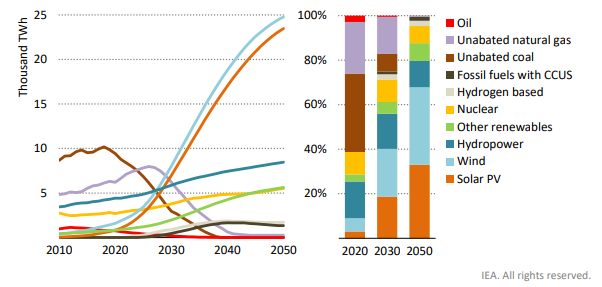
\includegraphics[width=0.8\textwidth]{Recursos/Imagenes/Graficas/NZE2050.png} \par\medskip
	
	\raggedright
	\footnotesize \textit{Nota.} Gráfico adaptado del reporte Net Zero Emissions by 2050 \citep{IEA_NZE_2021}.
	\label{fig:TendenciasNZE2050}
\end{figure}



En el ámbito nacional, la demanda energética peruana crece a un ritmo promedio anual de entre 3\,\% y 3.5\,\%, aunque con una profunda disparidad regional que contrasta el incremento del 26\,\% en la zona centro con severas contracciones en el norte (36\,\%) y sur (-18\,\%) \citep{ICEX2025}. En paralelo, la matriz de producción eléctrica, que alcanzó los 60 GW en 2024, avanza en su transición hacia fuentes limpias \citep{ProActivo2025}. Muestra de ello es que, para octubre de 2025, la generación mediante recursos renovables no convencionales (solar, eólica, bagazo y biogás) experimentó un crecimiento interanual del 27\,\%, representando el 13\,\% del total producido, en línea con el objetivo estratégico del Estado de alcanzar una participación del 20\,\% para el año 2030.

Las nuevas tendencias energéticas, lideradas por la tecnología solar fotovoltaica, plantean retos técnicos complejos para garantizar la eficiencia operativa \citep{XPower2024}. A medida que los proyectos fotovoltaicos escalan y se sitúan en terrenos topográficamente irregulares, factores como la variabilidad espacial de la irradiancia, las fluctuaciones térmicas, la suciedad y el ensombrecimiento afectan directamente la producción \citep{Salinas2025}. Bajo este escenario, la instrumentación rigurosa se convierte en un componente crítico. El despliegue estratégico de redes de sensores, equipos de diagnóstico y plataformas de monitoreo continuo es indispensable para determinar el índice de rendimiento (\textit{Performance Ratio}) bajo normativas como la IEC 61724 \citep{IEC61724-1_2021}. Esta precisión no solo es necesaria para validar el diseño de la planta frente a la variabilidad climática, sino que habilita estrategias de mantenimiento predictivo capaces de anticipar anomalías, minimizar tiempos de inactividad y asegurar el retorno de inversión, consolidando a la energía solar como una infraestructura económica y resiliente \citep{Anatrac}.

Sin embargo, para sostener este volumen de expansión, la industria solar se enfrenta a nuevas y complejas realidades geográficas para el emplazamiento de sus proyectos. Un número cada vez mayor de plantas fotovoltaicas a gran escala experimenta una transición hacia terrenos con topografía compleja y áreas montañosas, lo que genera una distribución espacial altamente fragmentada en el terreno \citep{Mao2025}.Esta nueva realidad montañosa cambia por completo cómo se comporta el viento en el lugar; las laderas actúan como una gran barrera física que frena y atrapa el aire en la parte más baja del terreno, mientras que hace que el viento acelere y sople con fuerza al llegar a la cima \citep{Xu2024}. Estas variaciones extremas en la velocidad del viento afectan directamente la enfriamiento de los paneles a lo largo del terreno, creando zonas con niveles de temperatura muy desiguales en la planta. 
La convergencia de estos flujos de aire irregulares, la alteración en la altura respecto al suelo y los patrones de sombras no uniformes crean un mosaico de microclimas muy distintos a lo largo de la instalación \citep{Armstrong2026}. En consecuencia, surge la necesidad ineludible de contar con herramientas dinámicas de diagnóstico que sean capaces de mapear estas variaciones espaciales del terreno, un desafío crítico que la instrumentación estática convencional es físicamente incapaz de resolver.


\section{Definición de la problemática}

La implementación de instrumentación en plantas fotovoltaicas se enfrenta a un desafío logístico y técnico considerable: la heterogeneidad de las condiciones climáticas dentro de una misma instalación \citep{Salinas2025}. A medida que los proyectos a gran escala se asientan sobre terrenos con topografías complejas, como las vistas en la Figura \ref{fig:PlantaPeru}, se generan microclimas que provocan variaciones espaciales significativas. Por ejemplo, las diferencias de elevación alteran localmente los perfiles aerodinámicos del viento, mientras que las variaciones topográficas causan una distribución desigual de la radiación solar. Estudios en plantas de gran tamaño demuestran empíricamente que esta dispersión geográfica puede generar diferencias de hasta un 20\,\% en la irradiación diaria y fluctuaciones extremas superiores al 40\,\% a nivel horario, así como variaciones térmicas de 6 a 7 °C entre paneles separados dentro de una planta solar \citep{Garcia2014}. 




\begin{figure}[H]
	% Fuerza la alineación izquierda y quita los ":" después del número
	\captionsetup{justification=raggedright, singlelinecheck=false, labelsep=none}
	
	\caption[Imagen aérea de planta de energía solar en inmediaciones de la fábrica de cemento Yura, Arequipa.]{} 
	
	\textit{Imagen aérea de planta de energía solar en inmediaciones de la fábrica de cemento Yura, Arequipa.} \par\medskip
	
	\centering
	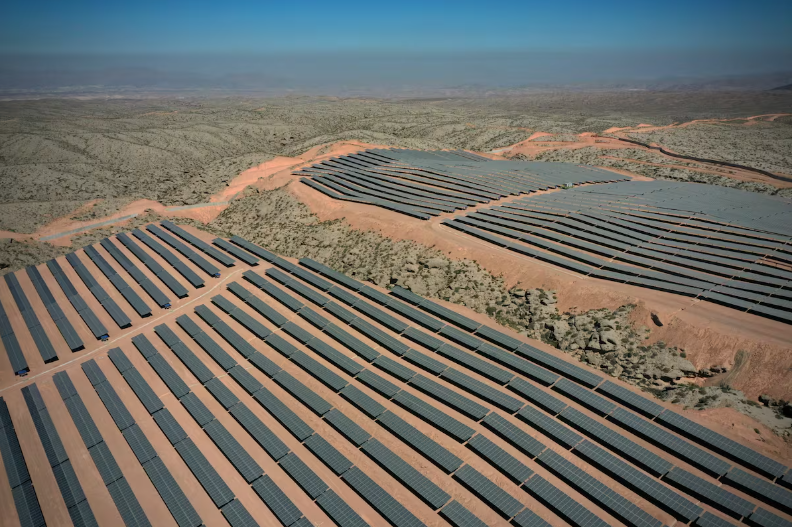
\includegraphics[width=0.6\textwidth]{Recursos/Imagenes/Otros/PlantaPeru.png} \par\medskip
	
	\raggedright
	\footnotesize \textit{Nota.} Fotografía adaptada sobre la noticia ``Yura y el poder del sol'' \citep{YuraPeru}.
	\label{fig:PlantaPeru}
\end{figure}


Para hacer frente a esta variabilidad y cumplir con los requisitos de monitorización de normativas internacionales, como la IEC 61724-1 \citep{IEC61724-1_2021}, las plantas recurren actualmente a la instalación de estaciones meteorológicas y redes de instrumentación fijas. En el contexto de un parque fotovoltaico, una estación meteorológica se concibe como un núcleo de monitorización centralizado mediante un adquisidor de datos, el cual integra una serie de instrumentos de alta precisión para caracterizar el recurso solar y el entorno climático \citep{Anatrac}. Típicamente, esta estación está equipada con piranómetros, sensores de temperatura ambiente, anemómetros y medidores de humedad relativa y presión atmosférica \citep{ProyectoEjecutivo2024}. Sin embargo, depender exclusivamente de puntos de medición estáticos presenta severas limitaciones. En la práctica, unos pocos sensores asumen un terreno plano y homogéneo, por lo que son físicamente incapaces de capturar con precisión la variabilidad climática real a lo largo de relieves montañosos y terrenos extensos \citep{Salinas2025}.

En consecuencia, el problema central se define como la ineficiencia de los métodos de instrumentación estáticos para caracterizar adecuadamente este mosaico de microclimas a lo largo de una planta fotovoltaica. Dado que los datos recopilados por la instrumentación fija no son verdaderamente representativos de las condiciones que experimentan los módulos en las distintas elevaciones del terreno, los operadores se enfrentan a una alta incertidumbre en la evaluación de los índices de rendimiento energético y a deficiencias importantes para la detección y localización oportuna de fallas operativas.

A esta falta de representatividad espacial se suma el enorme desafío financiero de intentar escalar o densificar la red de monitoreo instalando más estaciones fijas para cubrir el terreno. Adquirir y mantener múltiples estaciones meteorológicas de grado comercial representa un gasto logístico y económico notable, el cual puede llegar a constituir hasta el 1,6\,\% del presupuesto total de ejecución material de un proyecto fotovoltaico \citep{Burriana5MW}. Dado que resulta material y financieramente inviable instalar estos instrumentos fijos en cada zona del relieve, se evidencia la necesidad de transitar hacia métodos de inspección dinámicos y móviles que sean verdaderamente representativos de todo el entorno solar a un costo razonable.

\section{Propuesta de solución}

Para superar las limitaciones de la instrumentación estática, esta propuesta plantea el diseño y desarrollo de un robot móvil especializado en la medición de variables climáticas en plantas fotovoltaicas. A diferencia de la infraestructura fija, este sistema funcionará como una plataforma móvil adaptada para transportar instrumentos meteorológicos, lo que le permitirá realizar un barrido continuo y focalizado en diversas secciones de la planta. Al desplazarse estratégicamente por el terreno, el vehículo recolectará datos de alta resolución que reflejen con mayor exactitud la dispersión geográfica de la irradiancia, el mosaico de microclimas y las condiciones ambientales locales. Esto tiene el fin de reducir la incertidumbre en la estimación de la generación de energía, en cumplimiento con los métodos de evaluación exigidos por las normativas internacionales. Para complementar su funcionalidad, el sistema almacenará y transmitirá la información capturada de forma inalámbrica, facilitando una plataforma de monitoreo remoto donde los operadores podrán visualizar el estado ambiental de la instalación en tiempo real.


\subsection{Objetivos generales}

\subsubsection{Objetivo correspondiente a Trabajo de Fin de Carrera 1 (1MTR01)}
Elaborar el diseño conceptual y el anteproyecto de un robot autónomo para la medición dinámica de variables climáticas en sistemas fotovoltaicos, orientado a caracterizar la formación de microclimas y variaciones climáticas en la topografía.

\subsubsection{Objetivo correspondiente a Trabajo de Fin de Carrera 2 (1MTR02)}
Desarrollar la ingeniería de detalle, elaborar el proyecto definitivo e implementar un prototipo virtual del robot autónomo para la medición de variables climáticas en sistemas fotovoltaicos, validando de forma integrada su comportamiento cinemático, control autónomo y arquitectura de telemetría.

\subsubsection{Objetivo para el proyecto general}
Desarrollar, dimensionar y validar integralmente un sistema mecatrónico autónomo móvil para la monitorización e inspección de variables climáticas en plantas fotovoltaicas emplazadas sobre terrenos irregulares, culminando en el proyecto definitivo y su validación mediante prototipado virtual.

\subsection{Objetivos específicos}

\subsubsection{Objetivos correspondientes a Trabajo de Fin de Carrera 1 (1MTR01)}
\begin{itemize}
    \item Determinar los requerimientos funcionales, cinemáticos y de diseño del sistema mecatrónico a partir del análisis de las severas condiciones topográficas y la dispersión climática en los parques solares.
    \item Desarrollar el diseño conceptual del sistema de locomoción, identificando sus funciones mecánicas y seleccionando los principios de tracción óptimos para garantizar un desplazamiento estable sobre terrenos irregulares.
    \item Desarrollar el diseño conceptual del mecanismo articulado, abstrayendo sus requerimientos cinemáticos y de actuación para asegurar la orientación independiente y precisa de los sensores climáticos.
    \item Estructurar la lógica del sistema de control autónomo, definiendo las funciones de procesamiento de señales, navegación y actuación requeridas para el seguimiento de rutas y la evasión de obstáculos.
    \item Plantear la arquitectura para el subsistema de telemetría y comunicaciones para garantizar la transmisión confiable de datos entre el robot y la central de control.
    \item Seleccionar el concepto de solución óptimo del sistema mediante una evaluación técnico-económica de las diferentes alternativas planteadas.
\end{itemize}

\subsubsection{Objetivos correspondientes a Trabajo de Fin de Carrera 2 (1MTR02)}
\begin{itemize}
    \item Realizar el diseño de detalle mecánico y estructural del sistema de tracción y de la base articulada para orientación de la instrumentación meteorológica, seleccionando materiales normalizados y generando la planimetría de fabricación correspondiente.
    \item Diseñar el sistema electrónico, instrumentación de variables ambientales y la arquitectura de alimentación energética independiente, dimensionando el almacenamiento en baterías y los circuitos de acondicionamiento de señales.
    \item Desarrollar e implementar los algoritmos de control de navegación autónoma, seguimiento de trayectorias predefinidas y evasión de obstáculos en el entorno operativo de la planta solar.
    \item Diseñar y configurar la infraestructura de comunicación inalámbrica y la interfaz gráfica de telemetría para la supervisión remota y recepción de datos climáticos en tiempo real.
    \item Construir y validar el prototipo virtual del sistema mecatrónico mediante simulaciones dinámicas y cinemáticas multicuerpo, pruebas en lazo cerrado de control y análisis de tráfico de red.
    \item Elaborar el proyecto definitivo del sistema mecatrónico, incluyendo la lista exhaustiva de materiales (BOM), el presupuesto detallado de implementación, el análisis de costos y la planificación de los protocolos de mantenimiento preventivo y correctivo.
\end{itemize}

\subsubsection{Objetivos para el proyecto general}
\begin{itemize}
    \item Diseñar a detalle una base de transporte con alta capacidad de tracción, a partir del concepto mecánico seleccionado, para operar de manera estable sobre los terrenos irregulares que caracterizan a los parques solares.
    \item Diseñar una base móvil articulada e integrada al vehículo, basándose en la arquitectura óptima definida previamente, capaz de moverse y orientarse de forma independiente para adaptarse a la posición óptima requerida por los diversos sensores ambientales.
    \item Desarrollar un algoritmo de control autónomo, implementando la lógica estructurada en el diseño conceptual, que proporcione al vehículo la inteligencia necesaria para seguir rutas de inspección predefinidas y reaccionar ante imprevistos mediante la evasión de obstáculos.
    \item Implementar una infraestructura de comunicación inalámbrica, materializando el esquema tecnológico propuesto, y definir la interfaz de telemetría y control para garantizar que los datos recolectados lleguen al centro de control sin interrupciones y permitiendo la intervención manual remota.
    \item Elaborar el proyecto definitivo del sistema incluyendo la elaboración de la lista de materiales, la estimación total de costos de implementación y la planificación de los protocolos de mantenimiento.
\end{itemize}

\section{Alcance y limitaciones}
El alcance de este proyecto y sus delimitaciones operativas se definen en conjunto a través de las siguientes características:

\begin{itemize}
    \item Abarca el diseño de detalle y la implementación de un prototipo virtual de una base móvil robusta apta para desplazarse sobre los terrenos irregulares que caracterizan a las plantas fotovoltaicas.
    \item Incluye el desarrollo de la lógica y el algoritmo de control que permitirá al vehículo seguir rutas de inspección predefinidas y evadir obstáculos. No obstante, el desplazamiento se encuentra restringido por la morfología del suelo, limitando su operación a zonas con pendiente máxima del terreno de 16°.
    \item Comprende la incorporación de los instrumentos meteorológicos requeridos para monitorear las variables ambientales de forma dinámica. La precisión de esta instrumentación estará sujeta a factores ambientales, pudiendo verse mermada por el fenómeno del \textit{soiling} o presentar lecturas atípicas debido a sombras proyectadas y reflejos solares accidentales.
    \item La integridad mecánica, electrónica y de los sensores del sistema estará diseñada para soportar las altas exigencias climáticas de los parques solares, restringiendo su funcionamiento seguro a una temperatura ambiente máxima operativa de 45°C.
    \item Contempla la implementación de un sistema de telemetría para almacenar y transmitir los datos medidos, habilitando la supervisión y el control remoto. Su desempeño dependerá estrictamente de la cobertura y estabilidad de la red inalámbrica existente en la instalación. El alcance del proyecto se delimita estrictamente al diseño e implementación del robot móvil, o el nodo de la red de transmisión, a establecer el protocolo de red y definir la estructura de la interfaz de telemetría y control, garantizando que el robot sea capaz de interoperar con plataformas comerciales o estaciones base preexistentes en la planta fotovoltaica.
    \item La autonomía del robot estará directamente condicionada por la capacidad de su batería y su perfil de consumo energético, proyectándose una autonomía de operación continua de alrededor de 1 hora, lo que impone la necesidad de establecer ciclos de carga periódicos para mantener la continuidad del servicio en plantas que requieran un recorrido mayor al tiempo establecido.
\end{itemize}

\section{Metodología de diseño y desarrollo para TFC2} 

El desarrollo del sistema mecatrónico se rige rigurosamente por los estándares internacionales de diseño en ingeniería: la directriz \textbf{VDI 2221} \citep{VDI2221_2019}, la metodología de diseño sistemático de \textbf{Pahl \& Beitz} \citep{Pahl2007} y el estándar específico para sistemas mecatrónicos y ciber-físicos \textbf{VDI/VDE 2206} \citep{VDI2206_2021}. 

En la primera etapa (TFC1), se completaron las fases de clarificación de la tarea, análisis de requerimientos y diseño conceptual multidisciplinario, culminando en la selección del concepto de solución óptimo. Para el presente semestre (TFC2), la metodología se enfoca en la ingeniería de detalle, el prototipado virtual y la validación integral del sistema conforme al modelo en ``V'' de la VDI/VDE 2206, estructurándose en las siguientes etapas operativas:

\subsection{Planificación y requerimientos detallado}
En esta fase inicial se consolida la retroalimentación del anteproyecto de TFC1, se definen con precisión los objetivos específicos de TFC2, la metodología sistemática de trabajo, el índice preliminar unificado del documento y el cronograma de ejecución temporal.

\subsection{Diseño de detalle y dimensionamiento preliminar}
Comprende el cálculo cuantitativo y la determinación preliminar de las dimensiones del prototipo, la selección preliminar de actuadores de tracción y de orientación, sensores primarios y controladores embebidos, así como el desarrollo de los primeros esquemas cinemáticos, flujogramas de operación y diagramas de interconexión.

\subsection{Proyecto definitivo}
Constituye el núcleo del desarrollo técnico en todos los dominios de la ingeniería mecatrónica:
\begin{itemize} 
    \item \textbf{Dominio mecánico y estructural:} Selección final de materiales, análisis de esfuerzos estáticos y dinámicos, cálculo de transmisiones, diseño CAD 3D.
    \item \textbf{Dominio electrónico y de energía:} Diseño y esquemáticos de circuitos de potencia y control, ruteo de placas PCB, integración y acondicionamiento de los sensores meteorológicos, y dimensionamiento del banco de baterías y gestión energética.
    \item \textbf{Dominio de control y software embebido:} Programación y estructuración de los algoritmos de navegación, implementación de sensores, y rutinas de evasión de obstáculos y seguridad.
    \item \textbf{Dominio de comunicaciones y telemetría:} Configuración del protocolo de red inalámbrica, arquitectura cliente-servidor para la transmisión de datos climáticos y diseño de la interfaz gráfica de usuario para monitoreo remoto.
\end{itemize}

\subsection{Prototipado virtual, simulación y validación integrada}
Conforme a la directriz VDI/VDE 2206, se implementa un prototipo virtual tridimensional para la verificación del sistema completo. Se realizan simulaciones multicuerpo de la dinámica del vehículo sobre terrenos irregulares y pendientes de hasta 16°, validación en lazo cerrado de los algoritmos de navegación y control de orientación de sensores, y pruebas de concurrencia y latencia en la transmisión de paquetes de telemetría.

\subsection{Consolidación documental y evaluación económica}
Se culmina con la integración total de la documentación técnica: Lista de Materiales (BOM), presupuesto total y análisis de costos de implementación, manuales y plan de mantenimiento preventivo/correctivo.

